

\documentclass[10 pt]{beamer}
\usepackage[utf8]{inputenc}
%\usepackage[latin1]{inputenc}
%\usepackage[cyr]{aeguill}
\usepackage[T1]{fontenc}
\usepackage{graphicx}
\usepackage{amsmath,amsfonts,amsthm,amssymb}
\usepackage{algorithm}
\usepackage{algorithmic}
%\usepackage[]{algorithm2e}
\usepackage{hyperref}
\usepackage{color}
\usepackage{pstricks}
%\usepackage{stmaryrd}
%\usepackage{enumitem} 
\usepackage{bbm}
\usepackage{bm}
\usepackage{array}
\usepackage{relsize,exscale}
\usepackage{caption}
\usepackage{times}
\usepackage{subcaption}
\usepackage{graphicx} 
\usepackage{epstopdf}
\usepackage{tikz}
\usepackage{glossaries}
\usepackage{cancel}
%\usepackage{animate}
\setbeamersize{text margin left=0.2 cm}
  \setbeamersize{text margin right=0.2 cm}
  %\setbeamersize{sidebar width left=}
  %\setbeamersize{sidebar width right=taille}
%\usetikzlibrary{calc}
%\DeclareMathOperator*{\argmin}{argmin}


\definecolor{ao(english)}{rgb}{0.0, 0.5, 0.0}
\definecolor{armygreen}{rgb}{0.29, 0.33, 0.13}
\definecolor{britishracinggreen}{rgb}{0.0, 0.26, 0.15}
\definecolor{cadmiumgreen}{rgb}{0.0, 0.42, 0.24}
\definecolor{indigo}{rgb}{0.29, 0.0, 0.51}
\definecolor{lightgray}{gray}{0.85}
\definecolor{midnightblue}{rgb}{0.1, 0.1, 0.44}
\definecolor{burntorange}{rgb}{0.8, 0.33, 0.0}
\definecolor{royalblue}{rgb}{0.25, 0.41, 0.88}
\definecolor{darkmagenta}{rgb}{0.55, 0.0, 0.55}
\definecolor{byzantine}{rgb}{0.74, 0.2, 0.64}
\definecolor{blue-violet}{rgb}{0.54, 0.17, 0.89}
\definecolor{brown-traditional}{rgb}{0.59, 0.29, 0.0}
\definecolor{brown-web}{rgb}{0.65, 0.16, 0.16}
\definecolor{burgundy}{rgb}{0.5, 0.0, 0.13}
\definecolor{electricpurple}{rgb}{0.75, 0.0, 1.0}
\definecolor{gray}{rgb}{0.5, 0.5, 0.5}
\definecolor{goldenbrown}{rgb}{0.6, 0.4, 0.08}
\definecolor{armygreen}{rgb}{0.29, 0.33, 0.13}
\definecolor{calpolypomonagreen}{rgb}{0.12, 0.3, 0.17}
\definecolor{caputmortuum}{rgb}{0.35, 0.15, 0.13}
\definecolor{carmine}{rgb}{0.59, 0.0, 0.09}
\definecolor{chocolate-traditional}{rgb}{0.48, 0.25, 0.0}
\definecolor{lincolngreen}{rgb}{0.11, 0.35, 0.02}
\definecolor{magenta}{rgb}{1.0, 0.0, 1.0}
\definecolor{auburn}{rgb}{0.43, 0.21, 0.1}
\definecolor{bole}{rgb}{0.47, 0.27, 0.23}
\definecolor{bulgarianrose}{rgb}{0.28, 0.02, 0.03}
%\usepackage[dvipsnames]{xcolor}
%\xdefinecolor{vert_olive}{named}{OliveGreen}
%\xdefinecolor{bleuviolet}{named}{BlueViolet}
%\xdefinecolor{bleucadet}{named}{CadetBlue}
%\xdefinecolor{bleunuit}{named}{MidnightBlue}
\graphicspath{{./Figures/}}
\newtheorem{assumption}[theorem]{Assumption} 
\newtheorem{proposition}[theorem]{Proposition} 
\newtheorem{remark}[theorem]{Remark} 

\renewcommand{\div}{\mathrm{div}}
\newcommand{\Pdot}{\ddot{P}}
\newcommand{\Pdothn}{\Pdot_h^n}
%\usetheme{Madrid}
\usetheme{Frankfurt}

\title[SIAM GS 2019]{A hybrid parareal Monte-Carlo algorithm for the parabolic time
dependant diffusion equation}
\author[Jad Dabaghi]
{\underline{Jad Dabaghi}, Yvon Maday, Andrea Zoia}
\institute[]{Sorbonne Université \& CEA Paris Saclay}
\date{CANUM, December $3^{\mathrm{rd}}$ $2020$}
\subject{Numerical Analysis}
\newcommand{\nc}{\newcommand}

%%%%%%%%%%%%%%%

\nc{\Fdt}{\mathcal{F}_{\delta t}}
\nc{\FDT}{\mathcal{F}_{\Delta T}}
\nc{\GDt}{\mathcal{G}_{\Delta t}}
\nc{\GDT}{\mathcal{G}_{\Delta T}}

\newcommand{\matR}{\ensuremath{\mathbb{R}}}
\newcommand{\matN}{\ensuremath{\mathbb{N}}}
\newcommand{\matZ}{\ensuremath{\mathbb{Z}}}
\newcommand{\matX}{\ensuremath{\mathbb{X}}}

%%%%commandes principales

%\newcommand\egaldef{\stackrel{\mbox{\rm\tiny def}}{=}}
\newcommand{\beeq}{\begin{equation}}
\newcommand{\eeq}{\end{equation}}
\newcommand{\beeqn}{\begin{equation*}}
\newcommand{\eeqn}{\end{equation*}}


\newcommand{\guillemetright}{''}
\newcommand{\guillemetleft}{``}
\newcommand{\egaldef}{:=}
\nc{\myth}[1]{#1^{\scriptsize\mbox{th}}}
\nc{\lth}{\myth{l}}
\nc{\ith}{\myth{i}}
\nc{\dps}{\displaystyle}
\newcommand{\cf}{{\it cf.}}
\newcommand\ie{{\em i.e.}}
\newcommand\eg{{\em e.g.}}
%\nc{\tq}{{t.q}}
\renewcommand{\div}{\mathrm{div}}
\newcommand{\Mxl}{M_{\xl}}
\newcommand{\Ma}{M_{\ba}}
\newcommand{\Mal}{M_{\ba_l}}
\newcommand{\xl}{{\bm x}_l}
%%%%commandes ensembles entiers naturels, réels



%%%%%%

\newcommand{\vv}[1]{\ensuremath{{\bf #1}}}
\newcommand{\vu}{\vv{u}}

\newcommand{\dd}{\ensuremath{\mathrm{dt}}}
\newcommand\eal{{\em et al.}}
\nc{\tildef}{\tilde{f}}
\nc{\Mat}{\mathbf{M}}

\nc{\rla}{r_{\mathrm{l}, \ba}}
\nc{\rialfa}{r_{\ialf, \ba}}
\nc{\zialfa}{\zeta_{\ialf, \ba}}

\nc{\sialf}{s_{\ialf}}
\nc{\uialf}{u_{\ialf}}
\nc{\vialf}{v_{\ialf}}
\nc{\wialf}{w_{\ialf}}


\nc{\Id}{\mathrm{Id}}


\nc{\Ndpint}{\mathcal{N}_{\mathrm{d}}^{p,\mathrm{int}}}
\nc{\Ndofp}{\mathcal{N}_{\mathrm{dof}}^p}
\nc{\Ndp}{\mathcal{N}_{\mathrm{d}}^p}
\nc{\Vdp}{\mathcal{V}_{\mathrm{d}}^p}
\nc{\Vdpint}{\mathcal{V}_{\mathrm{d}}^{p,\mathrm{int}}}
\nc{\Vdpext}{\mathcal{V}_{\mathrm{d}}^{p,\mathrm{ext}}}
\nc{\Vdofp}{\mathcal{V}_{\mathrm{dof}}^p}
\nc{\Dofpint}{\mathcal{D}_{\mathrm{of}}^{p,\mathrm{int}}}
\nc{\Vdofone}{\mathcal{V}_{\mathrm{dof}}^1}
\nc{\Vdone}{\mathcal{V}_{\mathrm{d}}^1}
\nc{\Vj}{\mathcal{V}_j}
\nc{\Vjint}{\mathcal{V}_j^{\mathrm{int}}}
\nc{\Vjext}{\mathcal{V}_j^{\mathrm{ext}}}
\nc{\Vjmunint}{\mathcal{V}_{j-1}^{\mathrm{int}}}
%\nc{\Vhintprime}{\mathcal{V}_{h}^{int}}
%\nc{\Vhiipriment}{\mathcal{V}_{h-1}^{int}}


\nc{\Lah}{\Lambda_h}
\nc{\Lahp}{\Lambda_h^p}
\nc{\Lahone}{\Lambda_h^1}


\nc{\guna}{g_{\mathrm{1}}^{\ba}}
\nc{\gdeuxa}{g_{\mathrm{2}}^{\ba}}

%%%inconnues discrètes, linéarisés, muligrille

\nc{\bx}{{\bm x}}
\nc{\by}{{\bm y}}

\nc{\bu}{{\bm u}}
\nc{\bUk}{{\bm U}^k}
\nc{\bUki}{{\bm U}^{k,i}}
\nc{\bRki}{{\bm R}^{k,i}}
\nc{\br}{\bm r}
\nc{\bF}{{\bm F}}
\nc{\bB}{{\bm B}}
%\nc{\bC}{{\bm C}}
\nc{\bR}{{\bm R}}

\nc{\bb}{{\bm b}}

\nc{\bbD}{\mathbb{D}} 
\nc{\bbE}{\mathbb{E}} 
\nc{\bbG}{\bm{G}}
\nc{\bbGm}{\mathbb{G}} 
\nc{\bbK}{\bm{K}} 
\nc{\bbKm}{\mathbb{K}}
\nc{\bbS}{\mathbb{S}} 
\nc{\bbA}{\mathbb{A}} 
\nc{\bbAh}{\mathbb{A}_h}
%\nc{\bD}{{\bm D}}
%\nc{\bH}{{\bm H}}

\nc{\bphi}{{\bm \phi}}


\nc{\CFun}{{\bf C}}
\nc{\JacMat}[1]{{\bf J}_{#1}}
\nc{\JacCFun}{\JacMat{\CFun}}

\nc{\bs}{{\bm s}}
\nc{\bw}{{\bm w}}
\nc{\bv}{{\bm v}}
\nc{\uh}{{\bu}_h}
\nc{\vh}{{\bv}_h}
\nc{\X}{{\bm X}}
\nc{\Xh}{{\bm{X}}_h}
\nc{\bh}{{\bm b}_h}

\nc{\Xhki}{{\bm X}_h^{k,i}} \nc{\Xhkz}{{\bm X}_h^{k,0}} \nc{\Xhkiplusnu}{{\bm
X}_h^{k,i+\nu}}

\nc{\Xhkii}{{\bf X}_h^{k,i-1}}
\nc{\Xhk}{{\bm X}_h^k}
\nc{\Xhkminusun}{{\bm X}_h^{k-1}}

\nc{\uhk}{{\bm u}^{k}_h}

\nc{\ujhk}{u^{k}_{jh}}

\nc{\uhki}{{\bm u}_h^{k,i}}
\nc{\uhinfinf}{{\bm u}_h^{\infty,\infty}}
%\nc{\ujhki}{u^{k,i}_{jh}}

\nc{\uunhkminusun}{u^{k-1}_{1h}}
\nc{\uunhki}{u^{k,i}_{1h}}
\nc{\uialfhki}{u^{k,i}_{\ialf h}}
%\nc{\ulhki}{u^{k,i}_{lh}}

\nc{\uunhprimeki}{u^{k,i}_{1h'}}

\nc{\uun}{u_1}
\nc{\udeux}{u_2}


\nc{\uunhk}{u^{k}_{1h}}
\nc{\udeuxhk}{u^{k}_{2h}}
\nc{\uunhkmoinsun}{u^{k-1}_{1h}}
\nc{\udeuxhkmoinsun}{u^{k-1}_{2h}}

%% for non homogeneous BC
\nc{\uunhzero}{\hat{u}_{1h}}
\nc{\ghDir}{{\hat{g}}_h}

\nc{\Xk}{{\bf X}^k}



%%\nc{\rhki}{{\bf r}_h^{k,i}}
\nc{\Rhki}{{\bm R}_h^{k,i}}


%% domains
%\nc{\oma}{\omega_{\ba}}
\nc{\omaind}[1]{\omega_{#1}^{\ba}}
\nc{\omah}{\omaind{h}}
\nc{\omaj}{\omaind{j}}
\nc{\omajminusun}{\omaind{j-1}}



%%%%%espaces

\nc{\HdivOmeg}{ {\bf H}(\div,\Omega)}
\nc{\Hdivomeg}{ {\bf H}(\div,\omah)}
\nc{\Hdivomegj}{ {\bf H}(\div,\omaj)}
\nc{\Hdivomegjminusun}{ {\bf H}(\div,\omajminusun)}

\nc{\Pone}{\mathbbm{P}_1} 
\nc{\Pp}{\mathbbm{P}_p} 
\nc{\RTone}{{\bf RT}_1}
\nc{\RTp}{{\bf RT}_p}

%% Discrete Mixed Space
\nc{\Vspaceha}{{\bf V}_{h}^{\ba}}
\nc{\VTspaceha}{\widetilde{\bf V}_{h}^{\ba}}
\nc{\Qspaceha}{Q_{h}^{\ba}}
\nc{\QTspaceha}{\widetilde{Q}_{h}^{\ba}}

%% Discrete Mixed Space Multilevel case
\nc{\XXhp}{X_{h}^p}
\nc{\XXh}{X_{h}}
\nc{\Xhone}{X_{h}^1}

\nc{\Xgh}{X^{g}_{h}}
\nc{\Xghp}{X^{p}_{gh}}
\nc{\Xghone}{X^{1}_{gh}}

\nc{\Xzeroh}{X^{0}_{h}}
\nc{\Xzerohp}{X^{p}_{0h}}
\nc{\Xzerohone}{X^{1}_{0h}}

\nc{\Xzeroof}[1]{{X}^{0}_{#1}} 
\nc{\Xzeroj}{\Xzeroof{j}}
\nc{\Xzerojminusun}{\Xzeroof{j-1}} 
\nc{\XzeroJ}{\Xzeroof{J}}
\nc{\Xzerozero}{\Xzeroof{0}}
%%%%%%%%%





\nc{\M}{\mathbb{M}}
\nc{\N}{\mathbb{N}}

\nc{\nab}{{\bm \nabla}}


\nc{\HunK}{H^1(K)}
\nc{\HunOmega}{H^1(\Omega)}
\nc{\HunzeroOmega}{H^1_0(\Omega)}
\nc{\HungOmega}{H^1_g(\Omega)}
\nc{\HunCalO}{H^1(\calO)}
\nc{\HunzeroCalO}{H^1_0(\calO)}


%\nc{\norm}[1]{\Vert #1 \Vert}
\nc{\norm}[1]{\left\| #1 \right\|}
\nc{\normLtwo}[1]{\norm{#1}_{\Omega}}


\nc{\tnorm}[1]{\left| \hspace*{-0.12em} \left\| #1 \right\| \hspace*{-0.12em} \right|}


\nc{\calO}{\mathcal{O}}
\nc{\calC}{\mathcal{C}}
\nc{\calS}{\mathcal{S}}


\nc{\ialf}{\alpha} % index membranes

\nc{\Shko}{{\bf S}_h^{k,0}}
\nc{\Shkinnu}{{\bf S}_h^{k,i+\nu}}
\nc{\Rhkinnu}{R_h^{k,i+\nu}}
\nc{\Rhkii}{R_h^{k,i-1}}

\newcommand{\Proj}{{\bm{\Pi}}}
\newcommand{\ProjPone}{\Proj_{\Pone}}
\newcommand{\ProjPp}{\Proj_{\Pp}}
\newcommand{\ProjPoneK}{\Proj_{\Pone(K)}}
\newcommand{\ProjPoneTh}{\Proj_{\Pone(\Th)}}

%% hat functions \psi
\nc{\psih}[1]{\psi_{h,#1}}
\nc{\psiha}{\psih{\ba}}
\nc{\psihap}{\psih{\ba^\prime}}
\nc{\psihanum}[1]{\psih{\ba_{#1}}}
\nc{\psihal}{\psihanum{l}}
\nc{\psiham}{\psihanum{m}}
\nc{\psihl}{\psi_{h,\bx_l}}
\nc{\psihlstar}{\psi_{h,\bx_l^{*}}}
\nc{\Psihl}{\Theta_{h,\bx_l}}
\nc{\Psihlstar}{\Psi_{h,\bx_l^{*}}}
\nc{\psinum}[2]{\psi_{#1,#2}}
\nc{\psij}[1]{\psinum{j}{#1}}
\nc{\psija}{\psij{\ba}}
\nc{\psijal}{\psij{\ba_l}}
\nc{\psijmun}[1]{\psinum{j-1}{#1}}
\nc{\psijmuna}{\psijmun{\ba}}
\nc{\psijmunal}{\psijmun{\bal}}



%\newcommand\eal{{\em et al.}}


\nc{\CPF}{C_{\mathrm{PF}}}
\nc{\CPW}{C_{\mathrm{PW}}}
\nc{\CcontPF}{C_{\mathrm{cont},\mathrm{PF}}}
\nc{\Cst}{C_{\mathrm{st}}}

\newcommand\dv{\mathrm{div}}
\newcommand\Dv{\nabla {\cdot}}
\newcommand\Hdv{{\mathbf H}(\dv,\Om)}
\newcommand\Ho{H^1(\Om)}
\newcommand\Om{\Omega}
\newcommand\Hoo{H^1_0(\Om)}


%%%%%%%%%% Two phase flow

%%%%Phase and components
\nc{\liq}{\mathrm{l}}
\nc{\gas}{\mathrm{g}}
\nc{\water}{\mathrm{w}}
\nc{\hydro}{\mathrm{h}}

\nc{\phasel}{\mathrm{l}}
\nc{\phaseg}{\mathrm{g}}
\nc{\phasep}{p}
\nc{\componentd}{\mathrm{d}}
\nc{\componentc}{c}
\nc{\componentw}{\mathrm{w}}
\nc{\componenth}{\mathrm{h}}
\nc{\Cp}{\mathcal{C}^{\phasep}}
\nc{\Pc}{\mathcal{P}_{\componentc}}
\nc{\setcomponents}{\left\{\componentw,\componenth \right\}}
\nc{\setphases}{\left\{\mathrm{l},\mathrm{g}\right\}}
\nc{\Pcp}{P_{\mathrm{cp}}}
%%%%%%%%

%%% Continuous unknowns
\nc{\Qc}{Q_\componentc}
\nc{\Qw}{Q_{\mathrm{w}}}
\nc{\Qh}{Q_{\mathrm{h}}}

\nc{\Sp}{S^p}
\nc{\Sl}{S^{\mathrm{l}}}
\nc{\Sw}{S^{\mathrm{w}}}
\nc{\Sn}{S^{\mathrm{n}}}




%%%% Mesh and time simulation
\nc{\Th}{\mathcal{T}_h}
\nc{\Tind}[1]{\mathcal{T}_{#1}}
\nc{\Tj}{\Tind{j}}
\nc{\TJ}{\Tind{J}}
\nc{\Tjminusun}{\Tind{j-1}}
\nc{\Tz}{\Tind{0}}
\nc{\bn}{\bm n}
\nc{\Ptwo}{\mathbb{P}_2}
\nc{\Nhext}{N_h^{\mathrm{ext}}}
\nc{\card}{card \hspace {0.2cm}}
\nc{\Nt}{N_t}
\nc{\jump}[1]{\llbracket #1 \rrbracket} 
\nc{\Pm}{\mathbb{P}_m}
\nc{\PmcTh}{\mathbb{P}_m^{\mathrm{c}}(\Th)}
\nc{\PtwocTh}{\mathbb{P}_2^{\mathrm{c}}(\Th)}
\nc{\PonecOtF}{\mathbb{P}_1^{\mathrm{c}}(0,\tF)}

\nc{\PmdTh}{\mathbb{P}_m^{\mathrm{d}}(\Th)}
\nc{\PtwodTh}{\mathbb{P}_2^{\mathrm{d}}(\Th)}
\nc{\PzerodTh}{\mathbb{P}_0^{\mathrm{d}}(\Th)}

\nc{\Eh}{\mathcal{E}_h}

\nc{\DKmext}{D_K^{m,\mathrm{ext}}}
\nc{\DKm}{D_K^m}
\nc{\Dtwo}{D_{2}}
\nc{\Dm}{D_m}
\nc{\DKmint}{D_K^{m,\mathrm{int}}}
\nc{\Dmint}{D^{m,\mathrm{int}}}
\nc{\Dmext}{D^{m,\mathrm{ext}}}

\nc{\DKtwoint}{D_K^{2,\mathrm{int}}}
\nc{\VK}{\mathcal{V}_K}
\nc{\EK}{\mathcal{E}_K}
\nc{\EKint}{\mathcal{E}_K^{\mathrm{int}}}
\nc{\EKext}{\mathcal{E}_K^{\mathrm{ext}}}
\nc{\Ehint}{\mathcal{E}_h^{\mathrm{int}}}
\nc{\Ehext}{\mathcal{E}_h^{\mathrm{ext}}}
\nc{\Vh}{\mathcal{V}_h}
\nc{\ba}{{\bm a}}
\nc{\bal}{{\bm a_l}}
\nc{\oma}{\omega_{\bm a}}
\nc{\Nsp}{N_{\mathrm{sp}}}
\nc{\Ne}{N_{\mathrm{e}}}
\nc{\Dt}{\Delta t}
\nc{\dist}{\mathrm{dist}}
\nc{\tF}{t_{\mathrm{F}}}
\nc{\In}{I_n}
\nc{\Tn}{\tau_n}
\nc{\Ta}{\mathcal{T}_{\ba}}
\nc{\baprime}{{\bm a'}}


%% PHYSICAL UNITIES
\nc{\meter}{\mathrm{m}}
\nc{\kg}{\mathrm{kg}}
\nc{\yeer}{\mathrm{year}}

\nc{\icvg}{{\overline i}}
\nc{\kcvg}{{\overline k}} 


%%% Boltzmann

\nc{\MCS}{\Sigma_t}
\nc{\MCSS}{\Sigma_s}
\nc{\MCSA}{\Sigma_a}
\nc{\MCSF}{\Sigma_f}
%% mesh

\nc{\Nhint}{\mathcal{N}_h^{\mathrm{int}}}
\nc{\Vhint}{\mathcal{V}_h^{\mathrm{int}}}
\nc{\Vhext}{\mathcal{V}_h^{\mathrm{ext}}}
\nc{\Nh}{\mathcal{N}_h}

%% bold

\nc{\bU}{\bm U}

%% measure

\nc{\dx}{dx}


\setbeamertemplate{navigation symbols}{}
\setbeamercovered{transparent}



\AtBeginSection[] {
    \begin{frame}
    <beamer>[noframenumbering]
        \frametitle{Outline}
        \tableofcontents[currentsection]
    \end{frame}
}


\begin{document}


\begin{frame}
\maketitle

\includegraphics[scale=0.2]{image/logo_sorbonne}
\hfill 
\includegraphics[scale=0.14]{image/CEA}

\end{frame}




\newcommand{\kk}{\textcolor{royalblue}{k}}
\newcommand{\ii}{\textcolor{burntorange}{i}}
\newcommand{\nuu}{\textcolor{burntorange}{\nu}}


\setcounter{tocdepth}{4}
\section{Introduction}

\begin{frame}
\defbeamertemplate*{footline}{infolines theme frame plus slide}{\setcounter{slidenumber}{\insertpagenumber}\addcounter{slidenumber}{-\insertframestartpage}\addcounter{slidenumber}{1}}
\frametitle{Motivation}
\hspace*{0.2 cm} \textcolor{red}{\textbf{Study the neutron transport in nuclear reactors}}
\\
\vspace*{0.2 cm}
\invisible<1>{
\textcolor{midnightblue}{\textbf{Model:}} Linear Boltzmann equation for the angular flux
\begin{equation*}
\partial_t {\bm \Psi}(t,\bx,\bv) + \bv \cdot \nab {\bm \Psi}(t,\bx,\bv) + \sigma(\bx,\bv) {\bm \Psi}(t,\bx,\bv) - \int_{\mathbb{R}^3} k(\bx,\bv,\bv^{\prime}) {\bm \Psi}(t,\bx,\bv^{\prime})\,\mathrm{d} \bv^{\prime} = 0
\end{equation*}
Balance between the neutrons that are created and that disappear in the
core.
\\
\vspace{0.2 cm}
\invisible<2>{
\begin{minipage}{0.4 \linewidth}
\begin{figure}
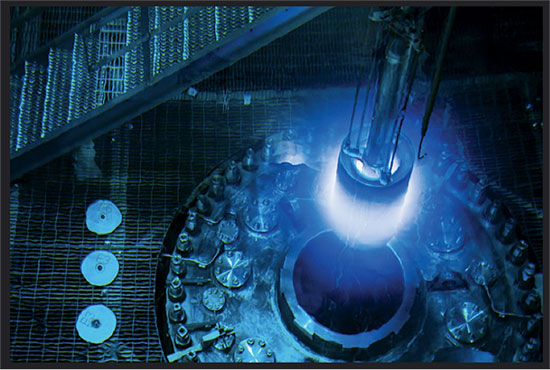
\includegraphics[scale=0.23]{image/reactor}
\end{figure}
\end{minipage}
\hfill
\begin{minipage}{0.55 \linewidth}

Numerical resolution:
\begin{itemize}
\item Monte-Carlo approach
\item Deterministic approach
\end{itemize}
\vspace*{0.2 cm}
Can we speed up a Monte-Carlo resolution?
\end{minipage}
\\
\vspace*{0.2 cm}
\invisible<3>{
\textcolor{cadmiumgreen}{\textbf{Parareal-in-time algorithm}} $\Rightarrow$ important computational savings
\begin{minipage}{0.2 \linewidth}
\begin{figure}

\includegraphics[scale=0.04]{image/attention}
\end{figure}
\end{minipage}
\hfill
\begin{minipage}{0.75 \linewidth}
Complicated problem... Start with a diffusion problem to understand the involved underlying mechanisms.
\end{minipage}
\invisible<4>{
  }}}}
\end{frame}

\section{Model problem}
    
\subsection{}  

\begin{frame}
\frametitle{Model problem and parareal algorithm}
\textcolor{cadmiumgreen}{\textbf{Time dependent diffusion equation with dirichlet boundary conditions:}}
\begin{equation*}
\dps
\left\lbrace\begin{array}{llccc}
\dps \partial_t u - \mathcal{D} \Delta u = g \quad & \mbox{in} \quad &\Omega \times \left[0,T\right], \\
 \dps u({\bm \cdot},0) = u^0 \quad & \mbox{in} \quad &\Omega,\\
u = 0 \quad & \mbox{on} \quad &\partial \Omega \times [0,T] . 
\end{array}
\right.
\end{equation*}
\invisible<1>{
\textcolor{cadmiumgreen}{\textbf{Parareal procedure:}}
It constructs a sequence $\bu_{\kk}^n:=(\bu_{\kk}^n)_{1 \leq n \leq N}$ such that $\bu_{\kk}^n \approx u^n$. It involves a coarse propagator $\GDt$ and a fine propagator $\Fdt$.\\
\vspace*{0.2 cm}
\invisible<2>{
\textcolor{cadmiumgreen}{\textbf{Coarse time grid discretization:}}
\begin{figure}
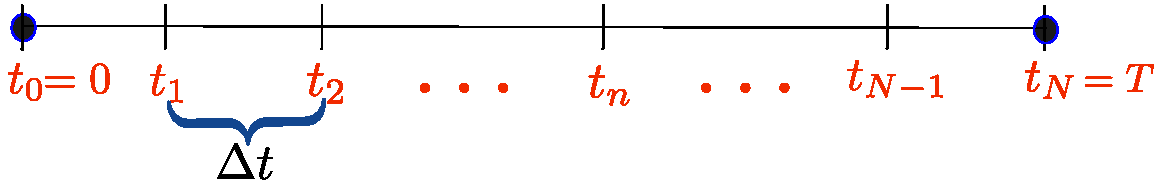
\includegraphics[width = 0.75 \textwidth]{image/discretization_time_coarse-cropped}
\end{figure}
 \invisible<3>{
\textcolor{cadmiumgreen}{\textbf{Fine time grid discretization:}}
 \begin{figure}
 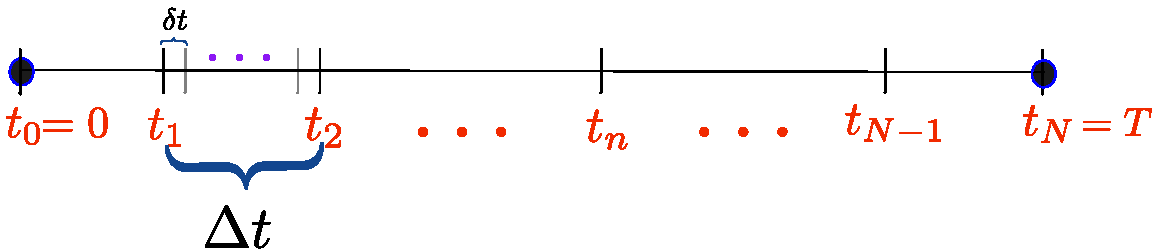
\includegraphics[width = 0.7 \textwidth]{image/discretization_time_coarse_fine_krop}
 \end{figure}
 \invisible<4>{
   }}}}
\end{frame}
%
\begin{frame}
\textcolor{midnightblue}{\textbf{The parareal algorithm}} 
\begin{equation*}
  \begin{split}
    u_{\kk=0}^{n+1} & := \GDt(u_{\kk=0}^n), \qquad \text{where} \quad u_{\kk=0}^0 := u^0. \\
    u_{\kk+1}^{n+1} & := \underbrace{\GDt(u_{\kk+1}^n)}_{\mathrm{prediction}} + \underbrace{\left[\Fdt(u_{\kk}^n) - \GDt(u_{\kk}^n) \right]}_{\mathrm{correction}}.
    \end{split}
\end{equation*}
\vspace{0.1 cm}
\invisible<1>{
\textcolor{midnightblue}{\textbf{Illustration of the procedure:}}
$n=4, \kk=2$

\invisible<2>{
1. Compute the coarse approximations:
\begin{equation*}
  u_{\kk=0}^{1}=\GDt(u^0), \quad u_{\kk=0}^{2}=\GDt^2(u^0), \quad u_{\kk=0}^{3}=\GDt^{3}(u^0)
\end{equation*}
\invisible<3>{
\hspace*{-0.15 cm} 
2. Compute: $u_{\kk \geq 1}^{1}=\Fdt(u^0)$ \\
\vspace*{0.1 cm}
\invisible<4>{
\hspace*{-0.05 cm} 3. Compute in parallel:
\begin{equation*}
  \Fdt(u_{\kk=0}^1) - \GDt(u_{\kk=0}^1), \ \Fdt(u_{\kk=0}^2) - \GDt(u_{\kk=0}^2), \ \Fdt(u_{\kk=0}^3) - \GDt(u_{\kk=0}^3)
\end{equation*}
\invisible<5>{
 4. \textcolor{cadmiumgreen}{\textbf{Update:}} $\fbox{$u_{\kk=1}^2$} \ \text{and} \ \GDt(u_{\kk=1}^2), \ \fbox{$u_{\kk=1}^3$} \ \text{and} \ \GDt(u_{\kk=1}^3), \ \text{and} \ \fbox{$u_{\kk=1}^4$} $
\\
\vspace*{0.2 cm}
\invisible<6>{
\hspace*{0.02 cm} 
5. Compute in parallel:
\begin{equation*}
\Fdt(u_{\kk=1}^1) - \GDt(u_{\kk=1}^1), \quad  \Fdt(u_{\kk=1}^2) - \GDt(u_{\kk=1}^2), \quad \Fdt(u_{\kk=1}^3) - \GDt(u_{\kk=1}^3)
\end{equation*}
\invisible<7>{
  6. \textcolor{cadmiumgreen}{\textbf{Update:}} 
 $ \fbox{$u_{\kk=2}^2$} \quad \text{and} \quad \fbox{$u_{\kk=2}^3$} \quad \text{and} \quad \fbox{$u_{\kk=2}^4$}$

\invisible<8>{
  }}}}}}}}
\end{frame}
%
\begin{frame}
  \frametitle{Coarse propagator}
  \vspace*{-0.1 cm}
  $\Th$: mesh of the domain $\Omega$\\
  \vspace{0.15 cm}
  $\Vh$ : Lagrange nodes, $\Vhint$: interior nodes, \\
  \vspace{0.15 cm}
  $\Nhint$ : number of internal Lagrange nodes, \ $\Nsp$ : number of elements \\
  \vspace*{0.15 cm}
\invisible<1>{
  \textcolor{midnightblue}{\textbf{The finite element propagator}}
  \begin{equation*}
    \begin{split}
X_h^p &:= \left\{v_h \in \mathcal{C}^{0}(\Omega); v_h|_{K} \in \mathbb{P}_p(K) \ \forall K \in \Th \right\} \subset H^1(\Omega) \\
X_{0h}^p & := \left\{v_h \in \mathcal{C}^{0}(\Omega); v_h|_{K} \in \mathbb{P}_p(K) \ \forall K \in \Th, \ v_h|_{\partial \Omega}=0 \right\} \subset H_{0}^1(\Omega)
\end{split}
  \end{equation*}
  
  The discrete vector of unknowns : $\bU_h^n \in \R^{\Nhint}$ satisfies $\bU_h^n = \GDt(\bU_h^{n-1})$ with
  \begin{equation*}
    \GDt(\bU_h^{n-1}) = [\mathbb{A}^n]^{-1}  \times \bF^{n-1}, \quad \underbrace{[\mathbb{A}^n]^{-1}}_{\mathrm{Stiffness} \ \mathrm{matrix} + \mathrm{mass} \ \mathrm{matrix}} \hspace{-0.6 cm} \in \R^{\Nhint,\Nhint}, \quad \bF^{n-1} \in \R^{\Nhint}
  \end{equation*}
  \vspace{-0.1 cm}
  \invisible<2>{
  \hspace*{-0.2 cm}\textcolor{midnightblue}{\textbf{The cell centered finite volume propagator}}
  \begin{equation*}
\bU_h^n \egaldef (\bU_K^n)_{K\in \Th}, \quad \textcolor{cadmiumgreen}{\textbf{one value per cell and time step}} 
\end{equation*}
  The discrete vector of unknowns : $\bU_h^n \in \R^{\Nsp}$ satisfies $\bU_h^n = \GDt(\bU_h^{n-1})$ with
  \begin{equation*}
    \GDt(\bU_h^{n-1}) = [\mathbb{A}^n]^{-1}  \times \bF^{n-1}, \quad \underbrace{[\mathbb{A}^n]^{-1}}_{\mathrm{Sparse}} \in \R^{\Nsp,\Nsp}, \quad \bF^{n-1} \in \R^{\Nsp}
  \end{equation*}
  \invisible<3>{
    }}}
\end{frame}
%
\begin{frame}
  \textcolor{midnightblue}{\textbf{The discontinuous Galerkin propagator}}
  \\
  \vspace*{0.2 cm}
  $\Nhint$:  total number of local internal degrees of freedom.
  \\
  \vspace*{0.2 cm}
  \textcolor{cadmiumgreen}{\textbf{Discontinuous Galerkin space:}}
  \begin{equation*}
    \begin{split}
      X_h^p & := \left\{v_h \in L^2(\Omega); v_h|_{K} \in \Pp(K) \ \forall K \in \Th  \right\} \not \subset H^1(\Omega),\\
X_{0h}^p & := \left\{v_h \in L^2(\Omega); v_h|_{K} \in \Pp(K) \ \forall K \in \Th, v_h|_{\partial \Omega} = 0  \right\} \not \subset H_0^1(\Omega)
    \end{split}
  \end{equation*}
  The discrete vector of unknowns : $\bU_h^n \in \R^{\Nhint}$ satisfies $\bU_h^n = \GDt(\bU_h^{n-1})$ with
  \begin{equation*}
    \GDt(\bU_h^{n-1}) = [\mathbb{A}^n]^{-1}  \times \bF^{n-1}, \quad [\mathbb{A}^n]^{-1} \in \R^{\Nhint,\Nhint}, \quad \bF^{n-1} \in \R^{\Nhint}
  \end{equation*}
  \textcolor{cadmiumgreen}{\textbf{local matrix}} $[\mathbb{A}^n]^{-1}_K = $ stiffness matrix $+$ mass matrix $+$ consistency and stability terms.
\end{frame}
%
\begin{frame}
  \frametitle{Fine propagator : Monte-Carlo}
  \textcolor{cadmiumgreen}{\textbf{Principle:}}
  It gives an approximation of
  \begin{equation*}
    \int_K u(\bx)\,\mathrm{d}\bx = \int_K \underbrace{f}_{PDF}(\bx) g(\bx)\,\mathrm{d}\bx.
  \end{equation*}
  \invisible<1>{
    Consider $M$ particles and sample a collection $X_1, X_2, \cdots, X_M$ of $M$ points from the PDF $f$. Denote by $\omega_i \in \R_{+}$ their statistical weight.
    \\
    \vspace*{0.2 cm}
    Compute $g(X_1)$,...,$g(X_M)$.
    \\
    \vspace*{0.2 cm}
  Then,
  \begin{equation*}
\int_K u(\bx)\,\mathrm{dx} = \overline{\mathbb{E}}\left[u(g(\bx))\right].
  \end{equation*}
    \\
    \vspace{0.2 cm}
    \invisible<2>{
  \textcolor{cadmiumgreen}{\textbf{Law of large numbers:}}
  \begin{equation*}
\lim_{M \rightarrow + \infty} \frac{1}{M} \sum_{i=1}^M g(X_i) = \int_K u(\bx)\,\mathrm{d} \bx.
  \end{equation*}
  \invisible<3>{
  \textcolor{cadmiumgreen}{\textbf{Central limit Theorem:}}
\vspace*{-0.15 cm}
  \begin{equation*}
    \mathrm{error} \approx 1/\sqrt{M}.
  \end{equation*}
  \invisible<4>{
    }}}}
\end{frame}
%
\begin{frame}
\frametitle{Sampling in 1D}


  \textcolor{cadmiumgreen}{\textbf{Direct inversion of the cumulative for a given PDF:}}
  \\
  \vspace*{0.2 cm}
  \invisible<1>{
$F : \Omega \rightarrow [0,1] \hspace{0.15 cm}$ such that $F(x) := \int_{- \infty}^{x} f(u)\,\mathrm{d}u$.
    \\ \vspace*{0.2 cm}
    Let $\xi_1 \sim \mathcal{U}([0,1])$.
    \\ \vspace*{0.2 cm}
    Position of the particle: ${X}_i=F^{-1}(\xi_1)$.
    \\ \vspace*{0.2 cm}
    Repeat $M$ times the procedure.
    \\
    \vspace*{0.3 cm}
    \invisible<2>{
    \textcolor{cadmiumgreen}{\textbf{The table lookup method:}}
    \\
    \vspace*{0.2 cm}
    Probability each element: $\mathbb{P}([x_{i-1},x_{i}]) = \int_{[x_{i-1},x_{i}]} f(x)\,\mathrm{d} x$,\\
    \vspace*{0.2 cm}
    Cumulative function: $F_{i}: \Omega \rightarrow [0,1], \ F_{i} = \sum_{j \leq i} \mathbb{P}([x_{j-1},x_{j}])$
    \\
    \vspace*{0.2 cm}      
    Let $\xi_1 \sim \mathcal{U}([0,1])$. Identify the two intervals such that $F_{i-1} \leq \xi_1 \leq F_{i}$. 
    \\
    \vspace*{0.2 cm}    
    Position of the particle: $\dps {X}_i = \frac{\left(x_i - x_{i-1}\right) \xi_1 - x_i F_{i-1} + x_{i-1} F_i}{F_i-F_{i-1}}$.
        \\ \vspace*{0.2 cm}
        Repeat $M$ times the procedure.
        \invisible<3>{
          }}}
\end{frame}
%
\begin{frame}
  \vspace{0.3 cm}
    \textcolor{cadmiumgreen}{\textbf{Rejection method:}}
    \\
    \vspace{0.1 cm}
    Often used when the PDF $f$ is hard to invert. Assume there exists a PDF $g : \Omega \rightarrow \R_{+}$ ``easy'' to simulate such that
    \begin{equation*}
f(x) \leq k g(x), \quad \text{where} \quad k \geq 1 \quad \text{is a constant}. 
      \end{equation*}
    Set $\dps \alpha(x)=\frac{f(x)}{k g(x)}$.
    \\
    \vspace*{0.2 cm}
    Compute the cumulative function $G:\Omega \rightarrow [0,1]$ associated to $g$.\\
    \vspace*{0.2 cm}
    Let $\xi \sim \mathcal{U}([0,1])$. \\
    \vspace*{0.2 cm}
    Find ${X}_i \in K$ using the direct inversion procedure.    \\
    \vspace*{0.2 cm}
    Compute $\alpha({X}_i)$.
    \\
    \vspace*{0.2 cm}
    Let $\xi_1 \sim \mathcal{U}([0,1])$. If $\xi_1 \leq \alpha ({X}_i)$ accept ${X}_i$. Otherwise reject and and come back to first step.
    \\
    \vspace*{0.3 cm}
    \textcolor{red}{\textbf{How define the transport of the particles?}}
\end{frame}
%
\begin{frame}
  \frametitle{Kernel Transport}
  $(\bx,t)$ : position of the particle $\bx$ at time $t$
  \\
  \vspace*{0.2 cm}
  $(\bx^{\prime},t^{\prime})$ : position of the particle $\bx^{\prime}$ at time $t^{\prime}$\\
  \vspace*{0.2 cm}
  Density transition kernel:
  \begin{equation*}
    T(\bx^{\prime},t^{\prime} \rightarrow \bx,t) :=
    \frac{1}{\sqrt{2 \pi \mathcal{D} \left(t-t^{\prime}\right)}}
    \exp \left(-\frac{(\bx-\bx^{\prime})^2}{2 \mathcal{D} \left(t-t^{\prime}\right)}\right).
  \end{equation*}
  %% \begin{equation*}
  %%   \bx - \bx^{\prime} \sim \mathcal{N}(\bx^{\prime}, \mathcal{D} (t-t^{\prime}))
  %% \end{equation*}
  \textcolor{cadmiumgreen}{\textbf{Pratical formula for the brownian motion:}}
  \begin{equation*}
T({\bm X}^{n+\delta t}, t^{n} + \delta t) = T({\bm X}^{n},t^{n}) + \sqrt{2 \mathcal{D} \delta t} \ \mathcal{S}_n \quad \text{where} \quad \mathcal{S}_n \sim \mathcal{N}(0,1)
    \end{equation*}
  \begin{figure}
    \centering
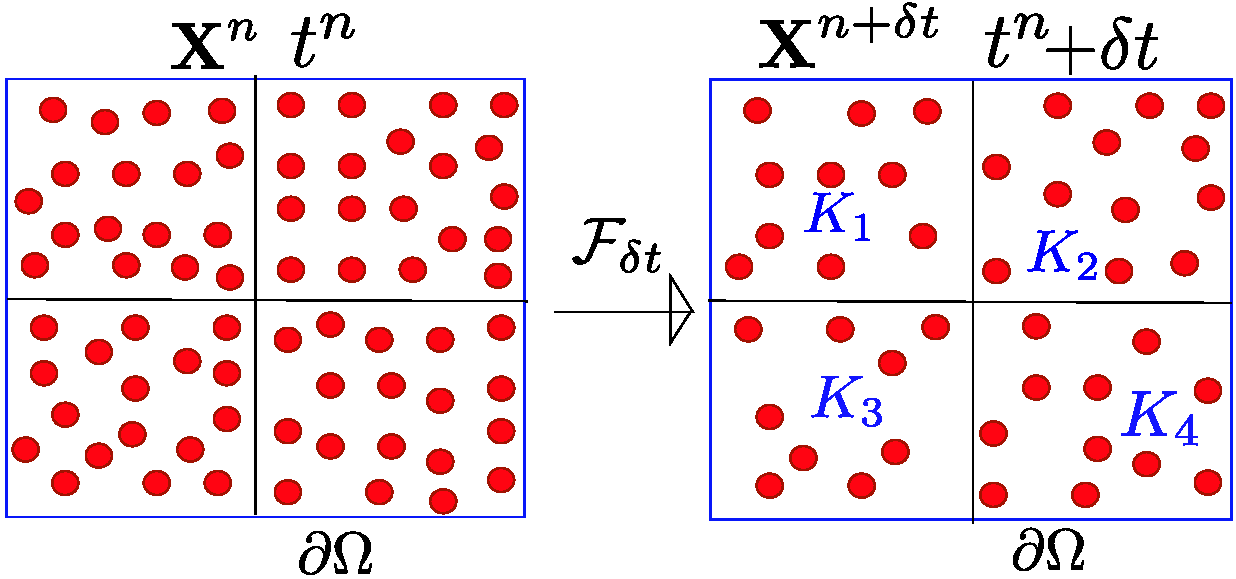
\includegraphics[scale=0.38]{image/Sampling_2D-cropped}
    \end{figure}
\end{frame}
%
\begin{frame}
\frametitle{Hybrid parareal algorithm}
\textcolor{midnightblue}{\textbf{Coarse propagator :}} Deterministic solver\\
\vspace*{0.2 cm}
\textcolor{midnightblue}{\textbf{Fine propagator:}} Monte-Carlo solver: deterministic data $+$ sampling $+$ average \\
\vspace*{0.2 cm}
Consider $p$ independent replicas and $M^{\prime}$ particles so that the total number of particles is $M = p \times M^{\prime}$.
The numerical solution obtained for a replica $j \in \left[1, p\right]$ at parareal iteration $\kk$ is denoted by ${\bm U}_{\kk,j}^{n+1}$
\begin{equation*}
{\bm U}_{\kk}^{n+1} := \frac{1}{p} \sum_{j=1}^p {\bm U}_{\kk,j}^{n+1}
\end{equation*}
\begin{minipage}{0.2 \linewidth}
\begin{figure}

\includegraphics[scale=0.04]{image/attention}
\end{figure}
\end{minipage}
\hfill
\begin{minipage}{0.75 \linewidth}
When ${\bm U}_{\kk,j}^{n+1}$ is computed, we need its statistical version for the computation of ${\bm U}_{\kk+1,j}^{n+2} = \GDt({\bm U}_{\kk+1,j}^{n+1}) \times \dps \frac{\textcolor{red}{\Fdt({\bm U}_{\kk,j}^{n+1})}}{\GDt({\bm U}_{\kk,j}^{n+1})}$. Introduce bias in the Monte-Carlo solver.
\end{minipage}
\end{frame}
%
\begin{frame}
  \frametitle{Updating the statistical weights}
  \textcolor{cadmiumgreen}{\textbf{Example:}} How avoid sampling ${\bm U}_{\kk=1}^2$?
  \begin{equation*}
[\omega_1^2]_{i\in K} = [\omega_{\mathcal{F}}]_{i \in K} \times \left(\frac{{\bm U}_{\kk=1}^2}{\mathcal{F}({\bm U}_{\kk=0}^1)}  \right)|_{K}
    \end{equation*}
  \begin{figure}
    \centering
    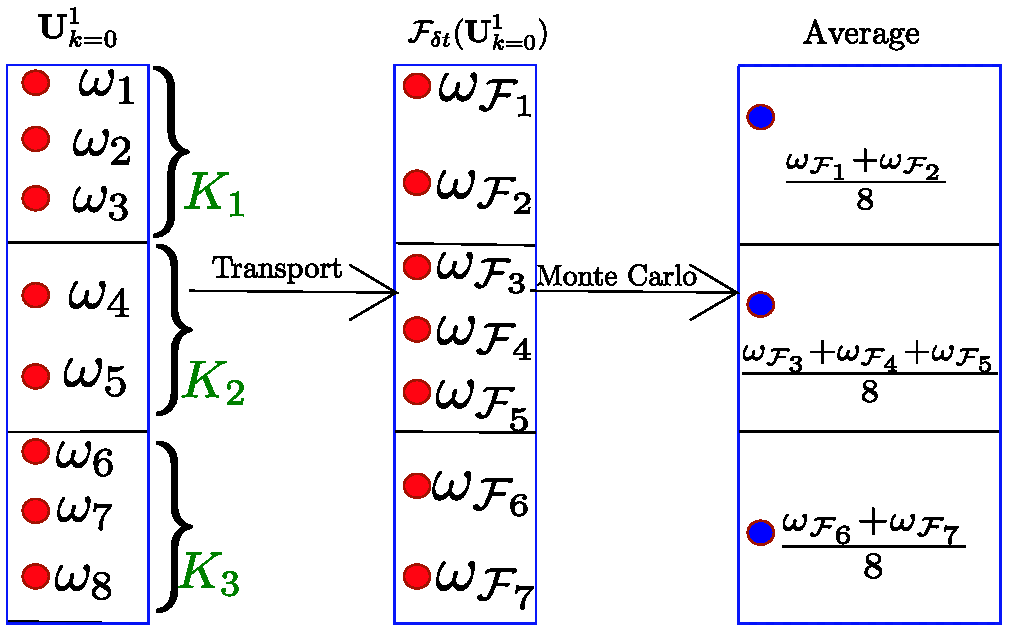
\includegraphics[scale=0.45]{image/reweighting-cropped}
  \end{figure}
  \begin{equation*}
    \mathrm{hist}(\omega_{\kk=1}^2)|_{K_1} = \frac{1}{8} \left(\omega_{\mathcal{F}_1} + \omega_{\mathcal{F}_2}\right) \times \left(\frac{{\bm U}_{\kk=1}^2}{\mathcal{F}({\bm U}_{\kk=0}^1)}\right)|_{K_1} = {\bm U}_{\kk=1}^2
  \end{equation*}
  \end{frame}

%
\section{Numerical experiments}
\subsection{}
\begin{frame}
\frametitle{Numerical experiments}
$\Omega$:  one-dimensional core with length $L = 5 m$, \textbf{Final simulation time:} $T=10 s$.
\\
\vspace{0.2 cm}
\textbf{Deterministic propagator:} $\mathbb{P}_1$ finite element, $\Delta t = 2 s$.
\\
\vspace{0.2 cm}
\textbf{Fine propagator:} Monte-Carlo, $\delta t = 2 \times 10^{-4} s$.
\\
\vspace{0.2 cm}
\textbf{Diffusion coefficient:} $\mathcal{D} = 0.5 m^2 \cdot s^{-1}$, \\
\vspace{0.2 cm}
\textbf{Initial condition:} $u_0(x)=\frac{1}{L}$.
\\
\vspace{0.2 cm}
\textbf{Number of particles:} $10^4$, \textbf{Number of replicas:} $10^3$
\\
\vspace{0.2 cm}
\begin{figure}
  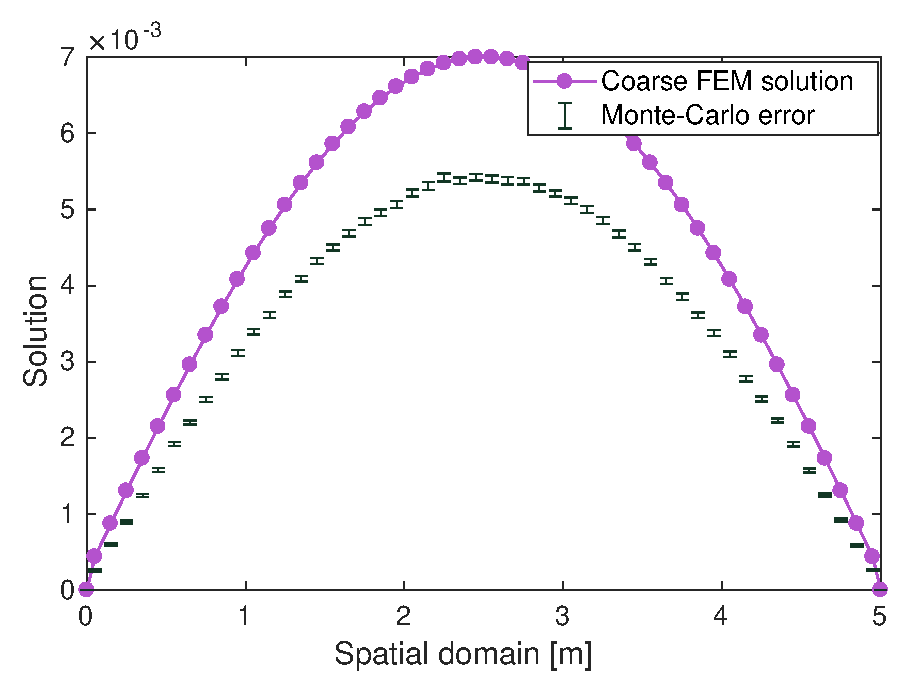
\includegraphics[width= 0.44 \textwidth]{image/Full_MC_coarse_FEM_n=8}
  \hfill
  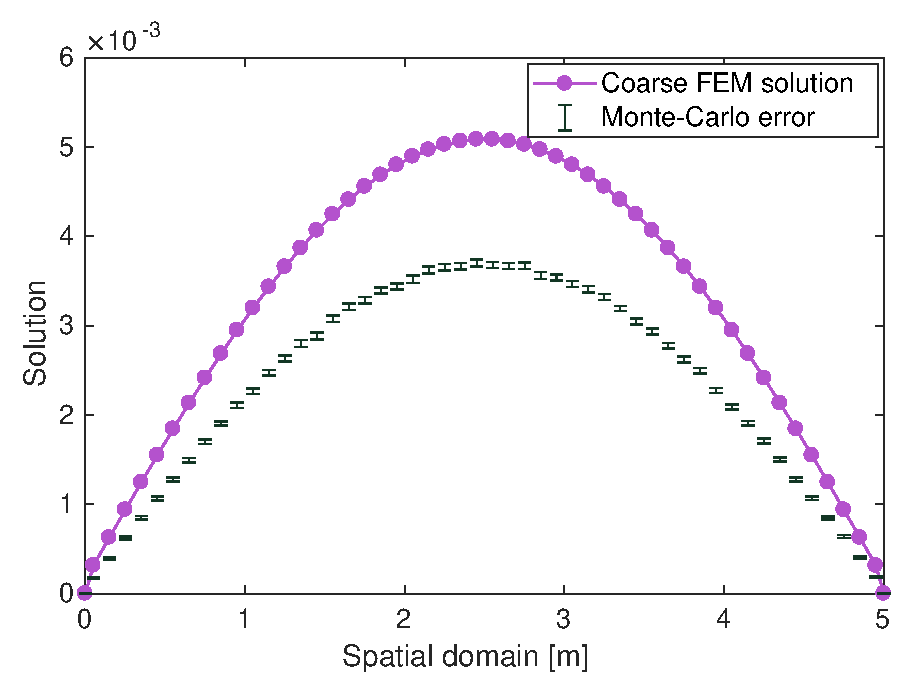
\includegraphics[width= 0.44 \textwidth]{image/Full_MC_coarse_FEM_n=10}
\end{figure}
\end{frame}
%
\begin{frame}
\frametitle{Hybrid solution}
  \begin{figure}
\centering
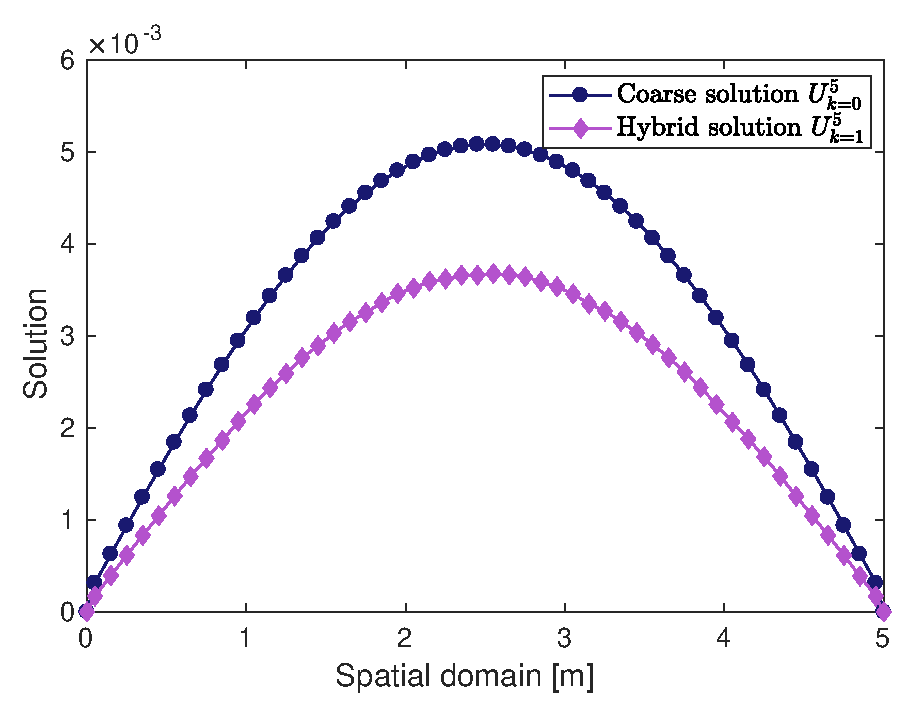
\includegraphics[width=0.49\textwidth]{image/Coarse_solution_vs_hybrid_n=5}
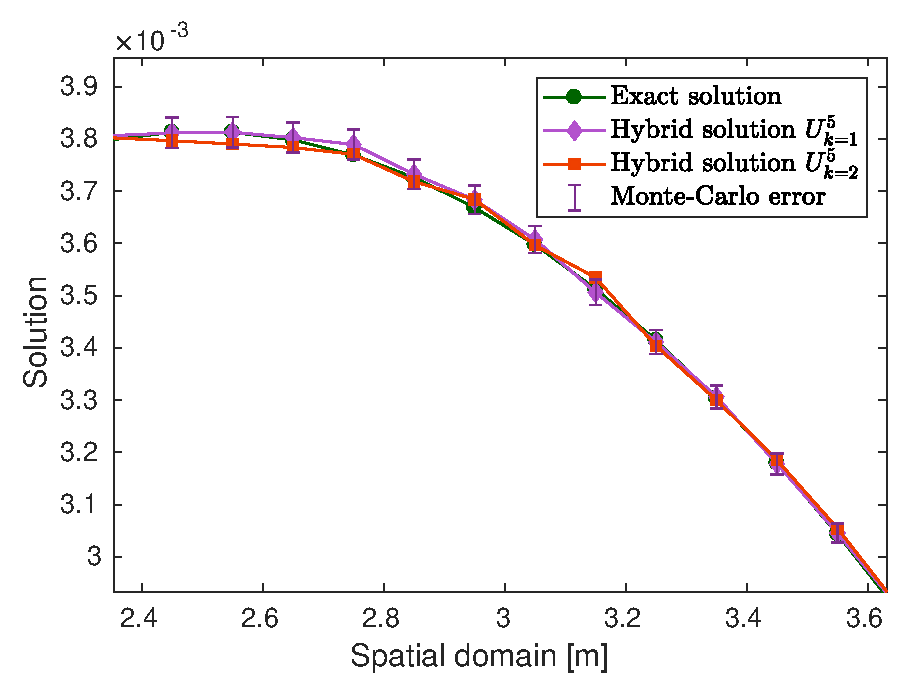
\includegraphics[width=0.49\textwidth]{image/hybrid_sol_MC_error_bar_zoom_bis} 
\end{figure}
\end{frame}
%
\begin{frame}
 \frametitle{CPU time and convergence}
\vspace*{-0.3 cm}
 \begin{figure}
\centering
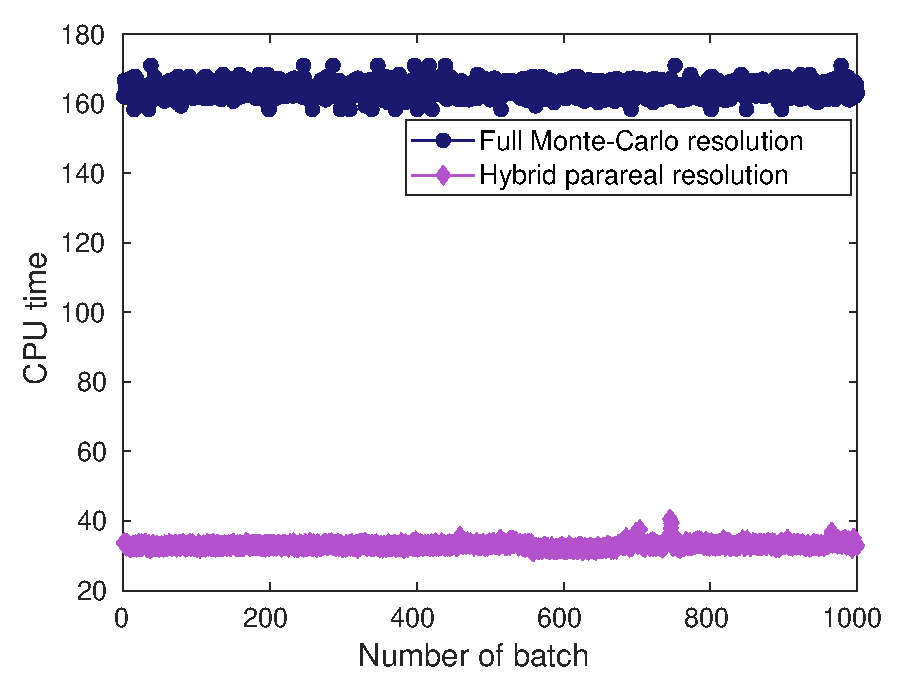
\includegraphics[width=0.48\textwidth]{image/CPU_time_hybrid_vs_MC}
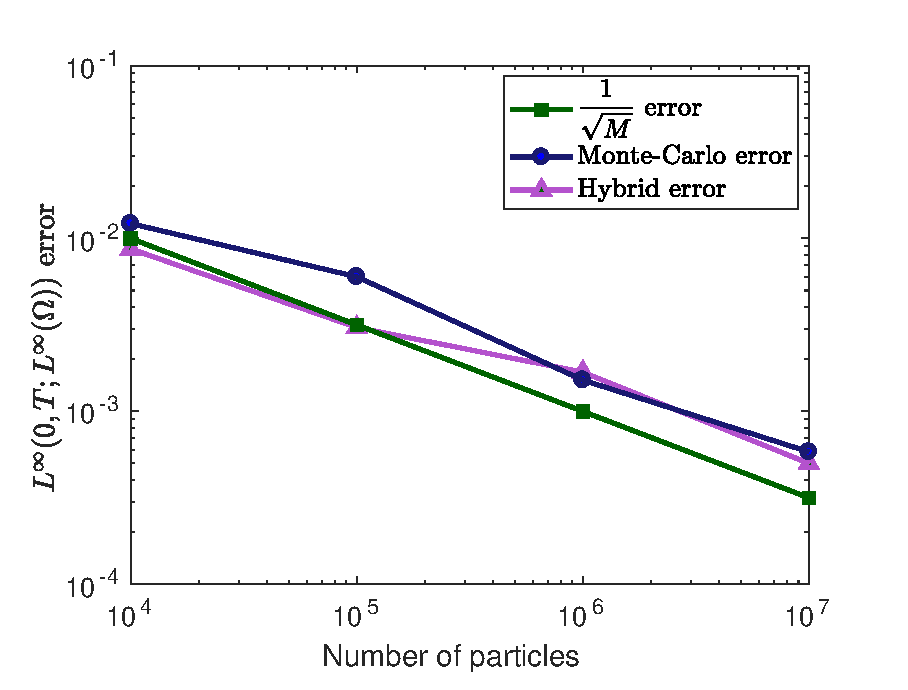
\includegraphics[width=0.5\textwidth]{image/Linf_error}
\end{figure}

\scriptsize
\begin{table}[]
\begin{tabular}{|c|c|c|c|c|c|c|l}
\cline{1-7}
\begin{tabular}[c]{@{}c@{}}Number \\ of \\ particles\end{tabular} & \begin{tabular}[c]{@{}c@{}}Number\\  of \\ replica \end{tabular} & \begin{tabular}[c]{@{}c@{}}Parallelized \\ Monte-Carlo\end{tabular} & \begin{tabular}[c]{@{}c@{}}Hybrid\\ parallelized\\ Monte-Carlo\\  $k=1$\end{tabular} & \begin{tabular}[c]{@{}c@{}}Hybrid\\ parallelized\\ Monte-Carlo\\ $k=2$\end{tabular} & \begin{tabular}[c]{@{}c@{}}Gain factor\\  $k=1$\end{tabular} & \begin{tabular}[c]{@{}c@{}}Gain factor\\ $k=2$\end{tabular} & \multicolumn{1}{c}{} \\ \cline{1-7}
$10^5$                                                            & $10^2$                                                        & $1653.4$ s                                                         & $335.76$ s                                                                           & $534.16$ s                                                                           & $4.92$                                                        & $3.04$                                                       &                      \\ \cline{1-7}
$10^4$                                                            & $10^3$                                                        & $164.09$ s                                                           & $33.05$ s                                                                             & $7.97$ s                                                                            & $4.96$                                                        & $3.09$                                                       &                      \\ \cline{1-7}
$10^3$                                                            & $10^4$                                                        & $16.86$ s                                                            & $3.39$ s                                                                             & $0.83$ s                                                                            & $4.97$                                                        & $3.07$                                                       &                      \\ \cline{1-7}
$10^2$                                                            & $10^5$                                                        & $1.78$ s                                                            & $0.35$ s                                                                             & $0.11$ s                                                                            & $5.08$                                                        & $3.02$                                                       &                      \\ \cline{1-7}
\end{tabular}
\end{table}
\end{frame}
%
\begin{frame}
  \frametitle{A second test case}
  \textbf{Final simulation time:} $T=14 s$.
\\
\vspace{0.3 cm}
\textbf{Deterministic propagator:} $\mathbb{P}_1$ finite element, $\Delta t = 2 s$.
\\
\vspace{0.3 cm}
\textbf{Fine propagator:} Monte-Carlo, $\delta t = 2 \times 10^{-4} s$.
\\
\vspace{0.3 cm}
\textbf{Diffusion coefficient MC:} $\mathcal{D} = 0.5 m^2 \cdot s^{-1}$
\\
\vspace{0.3 cm}
\textbf{Diffusion coefficient FEM:} $\mathcal{D}=0.48 m^2 \cdot s^{-1}$
\\
\vspace{0.3 cm}
\textbf{Initial condition:} $u_0(x)=\frac{1}{L} \left(1 + \cos(\frac{\pi x}{L}) \right)$.
\\
\vspace{0.3 cm}
\textbf{Number of particles:} $10^5$, \textbf{Number of replicas:} $10^2$
\end{frame}
%
\begin{frame}
  \frametitle{CPU time and convergence}
  \begin{figure}
\centering
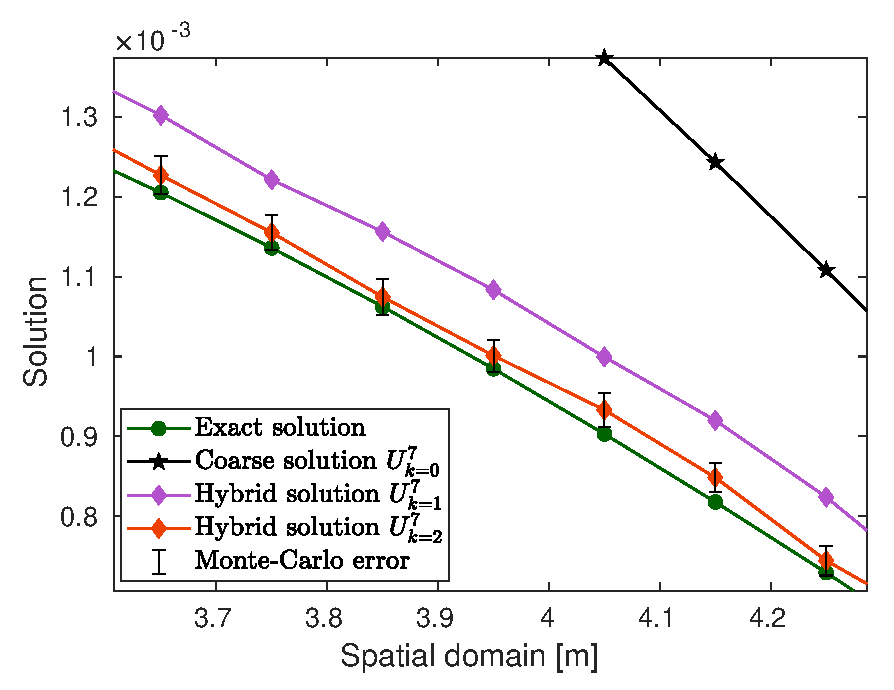
\includegraphics[width=0.49\textwidth]{image/sol_k1_k2_zoom}
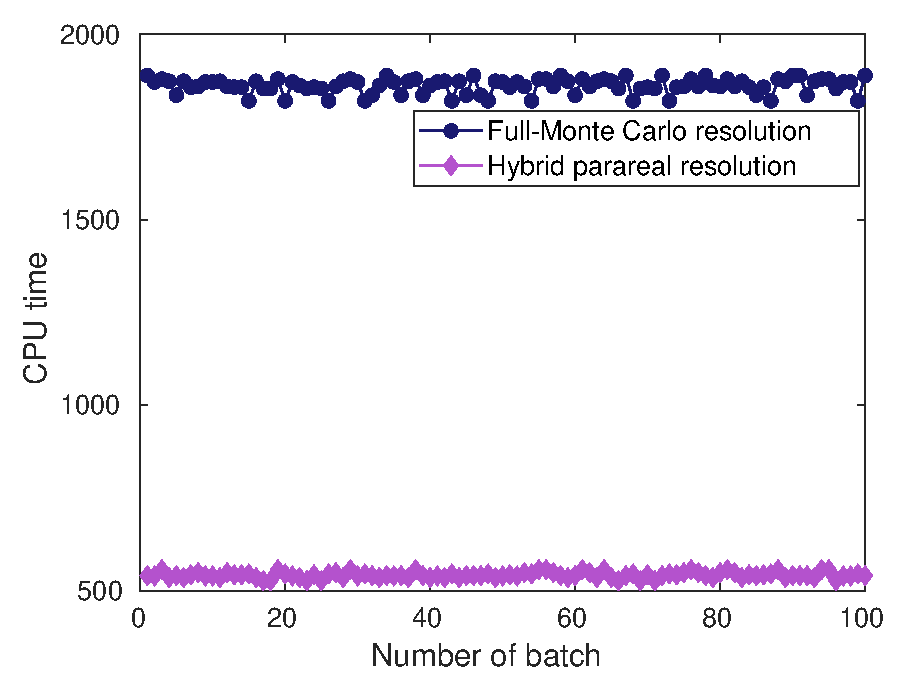
\includegraphics[width=0.5\textwidth]{image/CPU_time_trigo}
\end{figure}
\end{frame}
%
\section{Conclusion}
\begin{frame}
\frametitle{Conclusion}
\begin{itemize}
\item
We devised for the diffusion equation a hybrid parareal algorithm.
\vspace{0.3 cm}
\item Our approach reduces the CPU time of a Monte-Carlo simulation.
\end{itemize}
\vspace{0.5 cm}
\textcolor{red}{\textbf{Ongoing work:}}
\begin{itemize}
\item Extension to Boltzmann equation in neutronics
\end{itemize}
\vspace{0.5 cm}
\begin{thebibliography}{10}
 \scriptsize{
 \bibitem{Dabaghi:Maday:Zoia:2020}
 {\sc J.~Dabaghi, Y.~Maday, A.~Zoia, {\em A hybrid parareal Monte-Carlo algorithm for the parabolic
time dependant diffusion equation}.
 \textcolor{black}{In preparation}}}
 \end{thebibliography}

\end{frame}

\begin{frame}
\centering
\vspace*{1 cm}
\Huge Thank you for your attention!
\vspace*{2 cm}
\begin{figure}
\centering

\includegraphics[scale=1]{image/smiley}
\end{figure}
\end{frame}
%

\bibliographystyle{plain}
\bibliography{diphasique_biblio}
\end{document}



